\tightsection{Motivation and System Overview}
\label{sec:overview}

In this section, we present the motivation and an overview of our
system design.

The tenet of our work is that improving application performance in
today's Internet requires one to predict the outcome of different
decisions that the client or the server can make to optimize video
delivery. In order to predict these decision outcomes,
we argue for a global architecture that (1) continuously collects
performance information of ongoing sessions, and (2) use this
information to create an accurate \emph{model} that predicts the
performance of a session for a give configuration setting or protocol
decision (see Figure~\ref{fig:global-control--overview}). This
performance information can be collected at the client, at the server,
or at different network elements such as routers or caches. Predicting
the outcome of every possible decision enables us to make the best
decision, i.e., the decision that leads to the best outcome.

\begin{figure}[h!]
\centering
 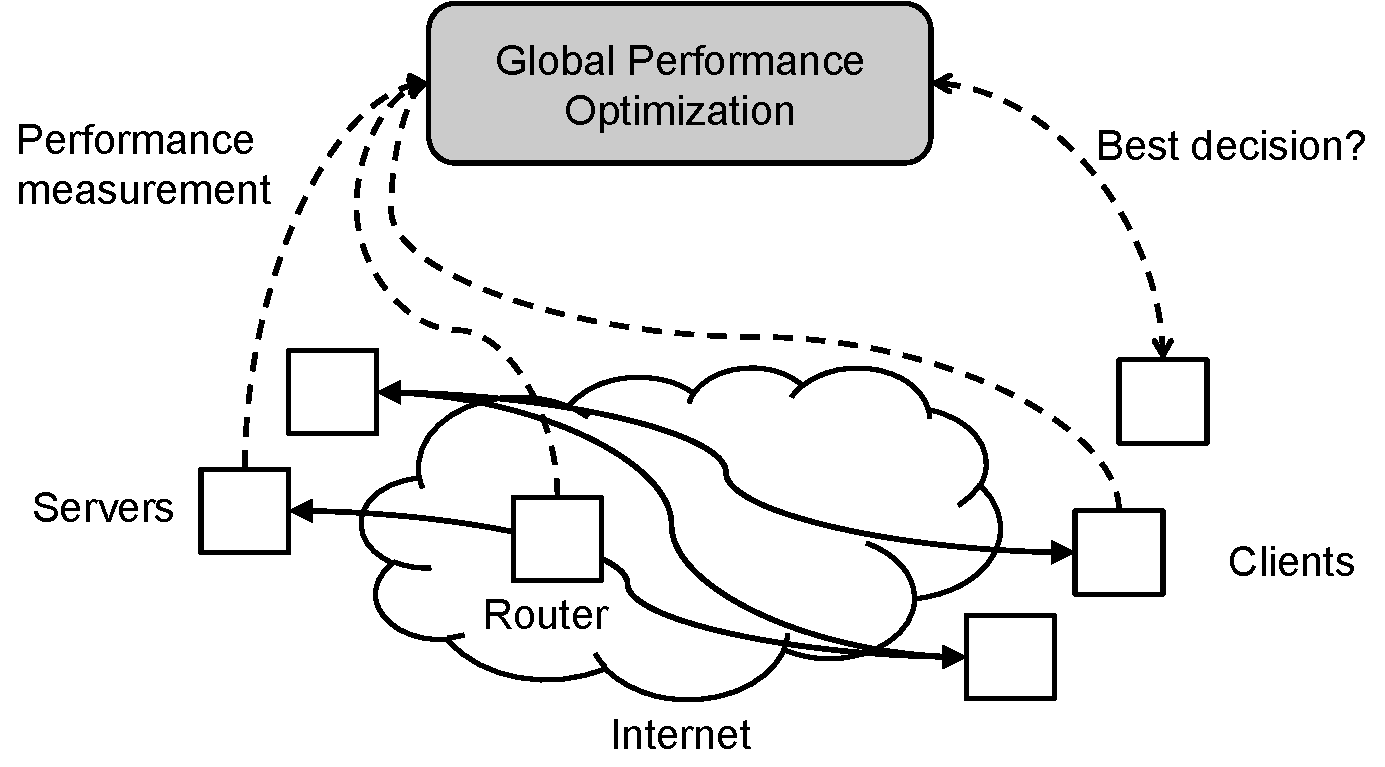
\includegraphics[width=0.5\textwidth] {figures/global-control-overview.pdf}
\tightcaption{Global performance optimization architecture.}
\label{fig:global-control--overview}
\end{figure}

\tightsubsection{Predictive Decision Model}

At the high level, any protocol designer aims to implicitly or
explicitly build a model of the environment (or world) in which the
protocol operates. Then the protocol takes the decision that optimizes
the utility of the predicted outcome.  For example, if it were
possible to predict whether packet loss would occur given a particular
TCP initial window size, we can maximize the QoS and user experience
by choosing the highest initial window size that wouldn't cause a
packet loss.  Similarly, if it were possible to predict whether a
client could sustain a particular bitrate, we can choose the highest
sustainable bitrate.

The challenge is to come up with a model that accurately describe the
world. Unfortunately, coming up with an analytical model of a complex
environment such as Internet is infeasible. As a result, we must use
direct measurements or observations of real world to inform our
model. This is the approach we take in this paper. In particular, we
use the performance of existing clients to predict the performance of
another client. For example, when a new client starts streaming a
video, we can use the quality experienced by other clients to predict
the quality that would be experienced by the new client when streaming
at a given bitrate. Based on this prediction, we can then select the
optimal bitrate for the new client.  In TCP protocol design, we might
gather data about many TCP connections to discover the distribution of
packet loss rates for different initial window sizes.  
%moved to related work \jc{Also cite
 % sigcomm'12 paper on data-driven TCP design which argues that TCP
 % parameters need to be driven by real data}

We refer to the resulting model\henry{need a different word for this;
  ``model'' is now unfortunately overloaded} of sharing information
across clients and making decisions based on predictions made by
shared information as a {\it predictive decision} model. 

% ION: move to discussion section
% We note that predictive decision model which requires sharing the
% information across clients at a global scale is naturally enabled by
% today's service architectures where a very large number of clients
% are typically connected to a backend at any given time. Google,
% Facebook, Microsoft, Yahoo!, and Twitter are just a handful of sites
% that can observe the quality and the performance experienced by a
% huge number users at any give time. Thus, maximizing the QoS of
% existing applications using predictive decision model does not
% require new architectures or building new large scale systems; it
% can be done in the context of the already existing artifacts.
% However, due to the complexity of networks -- in particular their
% temporal and spatial heterogeneity -- we find it is necessary to
% bring a degree of statistical sophistication to network modeling
% algorithms.


\tightsubsection{System Overview}

In this paper, we apply the idea of predictive decision model to video
quality optimization in the context of a large site that manages the
video delivery of many premium content brands such as HBO, MLB, and
ESPN. Video traffic is singularly important as it dominates the
Internet traffic today, and this domination will only intensify in the
forseable future.

As a first step in realizing the vision of the predictive decision and control 
platform, we have built a wide area distributed system, called video Global 
Optimization (GO). As shown in
Figure~\ref{fig:go-overview}, GO consists of two main components: (i)
a backend that collects and process the information about the video
quality across all clients, and (ii) a client library that collects
quality information at each client and sends it back to the backend. In
particular, the client library monitors the states of player and
network condition, summarizes them in the form of \emph{quality
  samples} (see details in \Section~\ref{subsec:dataset}) and send
these samples back to the GO backend.

\begin{figure}[h!]
\centering
 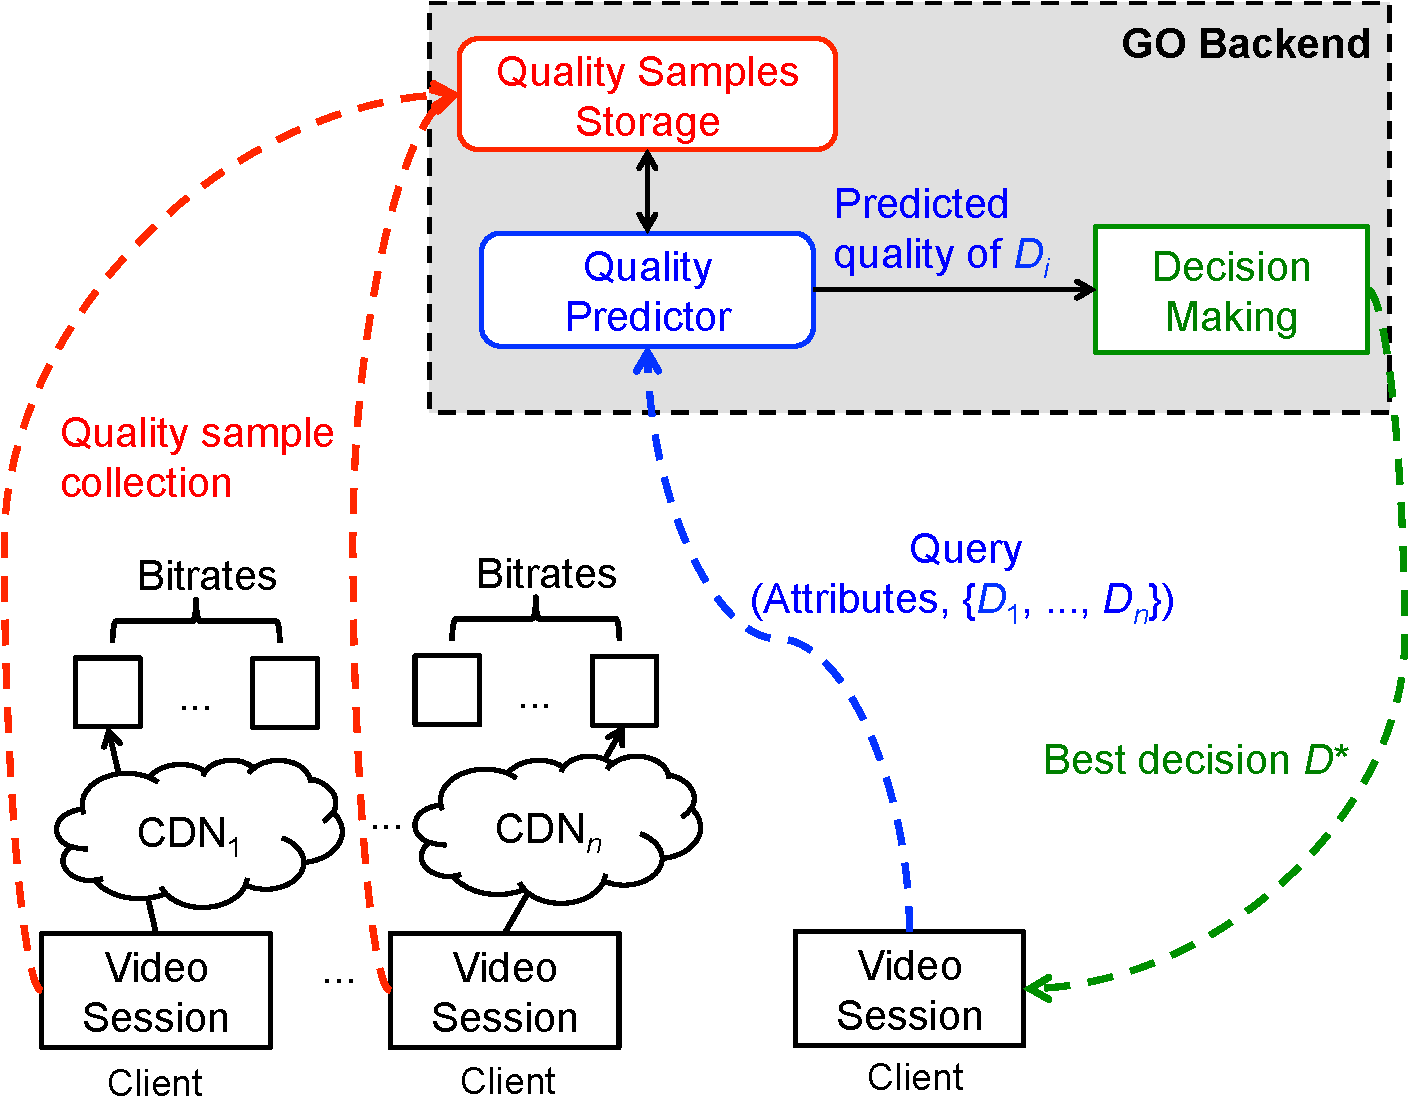
\includegraphics[width=0.5\textwidth] {figures/go-overview.pdf}
\tightcaption{Architecture of GO.}
\label{fig:go-overview}
\end{figure}
 
The GO backend uses a highly-scalable distributed streaming system to
process the quality samples received from clients, and predict the
quality outcomes of future sessions for each possible decision. There
are two decisions that GO makes: decide the {\it bitrate} of a session
(assuming the content is encoded at different resolutions), and decide
which CDN to stream the content from (assuming the content is stored
on multiple CDNs). The CDN and bitrate are chosen from a
pre-determined set of options and they can be changed at any point
during a session. Note that to play a video that is encoded at $n$
different bitrates and stored on $m$ CDNs, there are $m\times n$
options to chose from.  
%Readers may refer to~\cite{conext12} for more details.

To pick one of these options, GO predicts the quality metric for each
option, and then picks the one that corresponds to the highest
quality. In particular, GO uses real-time quality-related information
from every client currently streaming video to predict the quality of
another user if she were streaming from a particular CDN at a
particular bitrate, and use this prediction to select initial bitrate
and CDN for a new user.

%Since there are multiple quality metrics, GO combines them
%into a single figure of merit using a \emph{utility function}\jc{We do
%  not really use the notion of utility function now. Remember to echo
%  this point later on.}.  For example, a utility function may return a
%linear combination of several quality metrics.

It is worth noting that while current GO is limited in various dimensions,
we plan to extend GO to take more data and more control knobs in various 
part in the video delivery ecosystem.

\tightsubsection{Quality Samples} 
\label{subsec:dataset}

As explained above, the client library collects various quality
information, summarizes this information in quality samples, and send
these samples to the GO backend. More precisely, a quality sample
contains a set of quality measurements and attributes. Based on the
quality measurements, GO computes a set of quality metrics. In this
paper, we focus on four industry-standard video quality metrics that
have been shown to impact user's engagement~\cite{sigcomm11}:

\begin{packedenumerate}
\item \emph{Buffering ratio:} The percentage of time a session spends
  in buffering state, i.e., waiting for the player's buffer to
  replenish with enough data to continue the playback.
%Prior work has shown that buffering ratio is a key metric that impacts user engagement~\cite{sigcomm11}.
\item \emph{Join time:} The time it takes to start playing the video
  from the time the user clicks the ``play'' button.
% While join time may not directly impact the amount of a specific video viewed,
% it does have long term effects as it reduces the likelihood of repeated
%visits~\cite{sigcomm11,akamai-imc12}. 
\item \emph{Average bitrate:} Many of today's video players support
  adaptive bitrate switching to effectively react to changes in the
  bandwidth availability. The average bitrate of a session is simply
  the time-weighted average of the bitrates used in a given session.
%(Bitrate refers to the video playback rate, rather than throughput or download rate.)
\item \emph{Start failures:} Some sessions fail to start playing due
  to various reasons, including content unavailability, or CDN server
  overload.
% video; either the content is not available on the CDN server or the CDN is
%under overload or other unknown reasons. We mark as a session as a join failure
%if no content was played during this session.\footnote{Start failures are
%reported by the client-side measurement module that sends a ``heartbeat'' on
%the player status.}
\end{packedenumerate}

% Join time and start failures are valid metrics only for those
% sessions that just join the session.

In addition, a quality sample contains a large number of client and
video session attributes, including:

\begin{packedenumerate}
\item \emph{ASN:} The Autonomous System Number (ASN) that the client
  IP belongs to. Note that a single ISP (e.g., Comcast) may own
  different ASNs both for management and business reasons.

% We focus on the ASN as it is more fine-grained than the ISP
% granularity.  We observe in aggregate \fillme unique ASNs spanning
% multiple countries.

\item \emph{Object:} The video asset or object being streamed.
%We observe in aggregate \fillme objects.

\item \emph{Content provider (Site):} The video site providing the
  content. We have \fillme content providers that span different video
  genres.  We use the terms site and content provider interchangeably.

\item \emph{Initial CDN:} Thw CDN that the video session starts with.
  We see \fillme unique CDNs spanning popular CDN providers as well as
  several in-house and ISP-based CDNs. 
%(Some providers use proprietary
%  CDN switching logic; in this case we pick the segment of the session
%  with the CDN used for the longest duration.)

\item \emph{Initial Bitrate:} The bitrate the video session
  starts at. \fillme of the video objects we
  observe have multiple bitrates.

\item \emph{OS:} The OS of the client device, which in many cases
  determines the video player. For example, when watching the same
  video, iOS clients use different player than other OSes.

\item \emph{Connection type:} Type of the last mile connectivity,
  e.g., Wireless, DSL, fiber-to-home. This information is obtained
  from third party services~\cite{quova} based on the client's IP
  address.
\end{packedenumerate}


  In this paper, we report results from collecting quality samples
  from over \fillme million sessions or views (both successful and
  failed) over a duration of \fillme days.

%\myparasum{Previous research has shown prediction is necessary} In this context, video quality can be optimized by making the best decision (i.e., CDN, bitrate) for each session. Previous research \cite{sigcomm12,conext13} has provided insights on the potential of such optimization. In particular, it has shown (1) significant spatial diversity in CDN performance \footnote{CDN performance means the  overall video quality that viewers experience if the video is  streamed from it.} and availability across different geographical regions and ISPs; (2) substantial temporal variability in the CDN performance and client-side network performance; and (3) that causes of quality issues can be rooted in various attributes of a session (e.g., content provider, player implementation, or a combination). These results imply that there is no globally best decision which performs better than others for most sessions (in space) and for most of time (in time), and therefore, the best decision for any session should be made by predicting the video quality of each decision if it were to be used.


%\tightsubsection{Need of using client measurement} \jc{this subsection is logically needed, but not easy to argue.}

%In order to accurately predict the outcome of each decision, one
%approach is to have static models that characterize the quality of
%each decisions. However, this approach can be highly (1) complex as
%there are many entities that affect the quality along the path from
%video source to client in today's video delivery
%infrastructure~\cite{?}, and (2) costly to maintain as each session's
%quality may be affected by any factor. Alternatively\footnote{As also
%  argued in~\cite{sigcomm13DataDrivenTcp}}, we argue that by
%continuously collecting information about the performance of existing
%sessions, we will be able to predict the quality of new video sessions
%by looking at the performance of existing sessions that are close to
%it.

